Dette afsnit kommer til at handle omkring de overvejelser der har været omkring en brugergrænseflade, til dette projekts løsning. Her indgår også et livscyklus diagram, for hvordan brugergrænsefladen ser ud og ændrer sig, alt efter forskellige ting, såsom hvilken slags bruger der logger på. Den udgave af brugergrænsefladen, som blev valgt til at være grundmodellen for dette projekts løsning, vil også blive gennemgået og illustreret.

Til at starte med vil brugergrænsefladen for programmet være et almindeligt login vindue. Efter at et en bruger har indtastet et gyldigt brugernavn og password, vil programmet begynde at autentificere med en eventuel database. Alt efter hvilken slags type bruger som har logget på, så vil der blive hentet data fra databasen, som er tilknyttet den bruger som loggede på. Denne data vil herefter blive vist på brugerens grænseflade, som nu består af forskellige tabs, knapper osv.. Brugeren kan herefter interagere med denne data gennem brugergrænsefladen, indtil brugeren afslutter sessionen, hvor der til sidst vil blive synkroniseret med databasen, hvorefter programmet vil afslutte. Se på figur \ref{LifeCycle}.

\begin{figure}[H]
\centering
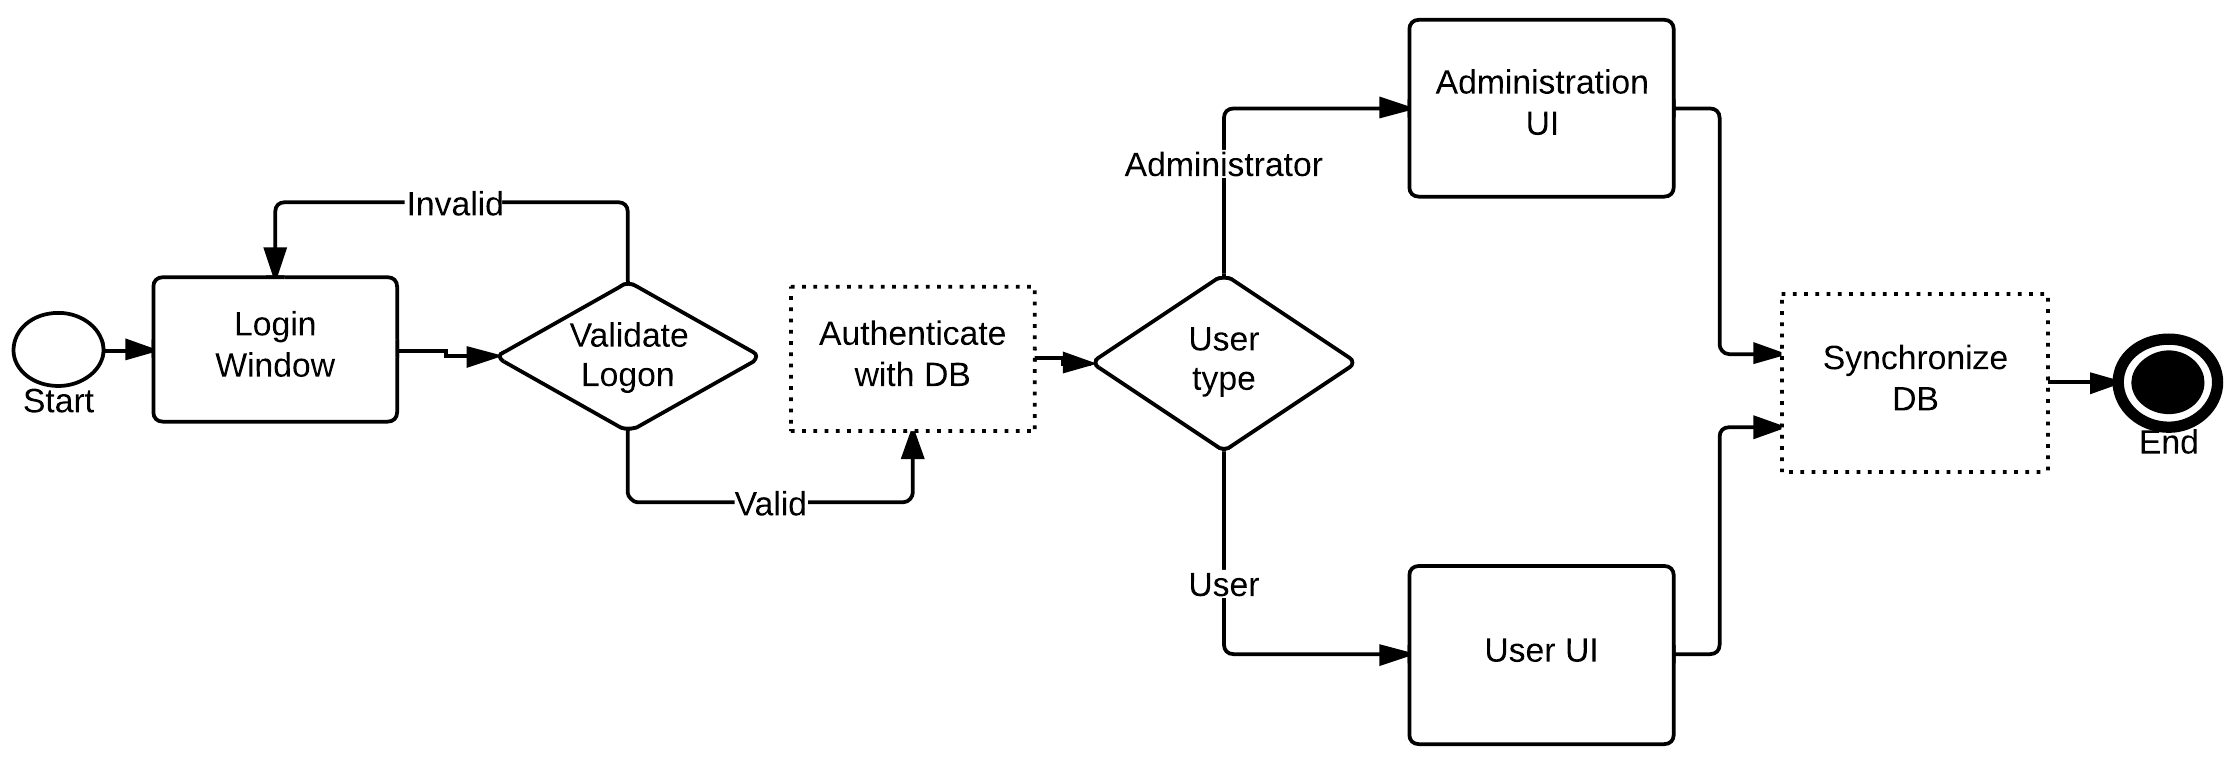
\includegraphics[width=1\textwidth]{Billeder/LifeCycle.png}
\caption{Brugergrænseflade/Program Livscyklus}
\label{LifeCycle}
\end{figure}